\chapter{Advanced transverse coupling measurement} 
 \label{sec_coupling}

\begin{chapterinfo}
    The compensation of the driven motion is necessary for a reliable coupling measurement.
    This chapter introduces methods to compensate for driven beam motion in the calculation of
    coupling resonance driving terms. The methods currently applied in the LHC are revised and
    recent findings are presented.
\end{chapterinfo}

\section{Driven coupled motion}
 In the past two methods were used for coupling measurements in
the LHC, the first one uses only the difference in tunes to rescale the coupling terms, this is
a naive approach because it disregards the driven betatron phase but often this approximation is
good enough to get a first estimate of the coupling in the machine. We refer to this method as the
\emph{model method}.

The second method \cite{Miyamoto2010} applies a detailled study of the driven particle motion and
provides a compensation for all optics parameters that enter into the coupling terms. This method will
be called \emph{formula method} in the following.

Recent findings \cite{Carlier2020} show that the AC-dipole locally effects RDTs and introduces
a jump at its location. The detailled considerations of the formula method lack such an effect.
In view of the suggestions of \cite{Carlier2020} this work presents calculations of the terms
$f_{1001}$ and $f_{1010}$, building upon the techniques introduced in \ref{sec_driven_coords}.
A comparison between model method, formula method and the newly calculated coupling terms are shown.


\subsection{AC-dipole as skew quadrupole}

To start the section about the beam motion that is driven \emph{and} coupled, we state a curious
analogy between AC-dipole and skew quadrupoles.

Throughout this chapter we use the following convention:
%
\begin{align}
    f_+ &\equiv f_{0101} \text{ and}\notag \\
    f_- &\equiv f_{0110} 
    \fstop
\end{align}
%
The RDTs in \eqref{eq_f0101_f0110} can be reformulated:
%
\begin{equation}
    f_\pm = 
    \frac{
        \sum\limits_w J_{1,w} \sqrt{\beta_{x,w}\beta_{y,w}}
        \e{
            i\left[\varphi_{wj,x} \pm \varphi_{wj,y}\right]
            -i\pi\left[Q_x\pm Q_y\right]
        }
    }{
        8i\sin[\pi(Q_x\pm Q_y)]
    }
    \fstop
\end{equation}
%
The coupled motion for a single coupling source now reads
%
\begin{align}
    h_x(s_j,N) =& \zxp(s_j,N) \notag \\
    &+2i\frac{
         J_{1,w} \sqrt{\beta_{x,w}\beta_{y,w}}
    }{
        8i\sin[\pi(Q_x + Q_y)]
    }
    \zyp(s_j,N)
        \e{
            i\left[\Delta\phi_x^+ + 2\pi Q_x \Theta(s_j,s_w) + 2\pi Q_y \Theta(s_j,s_w)\right]
            -i\pi\left[Q_x + Q_y\right]
        }
        \notag \\
    &+2i\frac{
         J_{1,w} \sqrt{\beta_{x,w}\beta_{y,w}}
    }{
        8i\sin[\pi(Q_x - Q_y)]
    }
    \zym(s_j,N)
        \e{
            i\left[\Delta\phi_x^- + 2\pi Q_x \Theta(s_j,s_w) - 2\pi Q_y \Theta(s_j,s_w)\right]
            -i\pi\left[Q_x - Q_y\right]
        }
        \komma
\end{align}
%
with 
%
\begin{equation}
    \Delta\phi_x^\pm = \varphi_x(s_j) - \varphi_x(s_w) \pm \left(\varphi_y(s_j) - \varphi_y(s_w)\right)
    \fstop
\end{equation}
%
The $\Theta(s_j,s_w)$ terms come from the wrapping around of the phase advance. Noting that 
$\zyp(s_j,N) = \sqrt{2I_y}\e{2\pi i N Q_y + \varphi(s_j)}$
one can bring this in a form similar to \eqref{eq_forced_motion}
%
\begin{align}
    h_x(s_j,N) =& \zxp(s_j,N) \notag \\
    &+\frac{
         J_{1,w} \sqrt{\beta_{x,w}\beta_{y,w}}
    }{
        4\sin[\pi(Q_x + Q_y)]
    }
    \sqrt{2I_y}
    \e{
        2\pi i N Q_y + \varphi(s_j)
        +i\left[\Delta\phi_x^+ + 2\pi (Q_x+Q_y) \text{sgn}(s_w-s_j)\right]
    }
        \notag \\
    &+\frac{
        J_{1,w} \sqrt{\beta_{x,w}\beta_{y,w}}
    }{
        4\sin[\pi(Q_x - Q_y)]
    }
    \sqrt{2I_y}
    \e{
        -2\pi i N Q_y + \varphi(s_j)
        +i\left[\Delta\phi_x^- + 2\pi (Q_x-Q_y) \text{sgn}(s_w-s_j)\right]
    }
    \fstop
\end{align}
%
The following table summarises which quantities get replaced
\begin{center}
\begin{tabular}{ll}
    AC dipole & coupling \\
    \hline
    \hline
    $ A_\theta $        & $ J_{1,w} $ \\
    $ \varphi_x(s_d) $  & $ \varphi_y(s_j) - \varphi_y(s_w) \mp \varphi_x(s_w)$ \\
    $ \Qd{x} $          & $ Q_y $\\
    \hline
\end{tabular}
\end{center}
Thus, a single coupling source acts like an AC dipole with the tune of the other plane as driving frequency.
From another perspective, the AC dipole couples the beam's motion to its oscillation.

\subsection{Derivation of the coupled driven motion}


The derivation of the coupled driven motion follows a similar path to the derivation of the 
coupled free motion but in the regime of driven motion, so the normal form approach has to be used.
Figure~\ref{fig_sketch_drv_ac} illustrates the procedure. The coordinates are propagated in normal form
space and transformed to physical space at $s_d-\epsilon$, directly in front of the AC-dipole. Then
an AC-dipole kick $\Delta h_x(N)$ is performed and the physical coordinate is transformed back to
normal form space where it is rotated around the ring. This process is repeated for each turn.

\begin{figure}
  \centering
  tikzpicture
      \caption{Kick performed in CS-coordinates, transformed to NF-coordinates}
  \label{fig_sketch_drv_ac}
\end{figure}

In the first turn, before the beam experiences the AC-dipole kick, the coordinates are those from
\eqref{eq_coupled_h_from_z}:
%
\begin{align}
  h_x^+(s_d-\epsilon, 0) &=  \e{\liemap{F}} \zeta_x^+(s_d-\epsilon, 0)\notag \\
  &=  \zeta^+(s_d-\epsilon,0)
    + 2i\conj{f_{1001}}\zeta_y^+(s_d-\epsilon, 0)
    + 2i\conj{f_{1010}}\zeta_y^-(s_d-\epsilon,0)
\end{align}
%
Then the particle is kicked in $p_x$ direction:
%
\begin{equation}
  h_x^+(s_d+\epsilon, 0) =  h_x^+(s_d - \epsilon,0) + \Delta h_x(0)
\end{equation}
%
For the transformation back to normal form space the inverse of \eqref{eq_h_from_z} has to be applied:
%
\begin{equation}
  \zeta = \e{\liemap{-F}} h = h + [-F,h] + O(h^3)
  \label{eq_coupled_h_after_kick}
\end{equation}
%
with
%
\begin{equation}
  F = \sum f_{jklm}\left( h_x^+ \right)^j \left( h_x^- \right)^k \left( h_y^+ \right)^l \left( h_y^- \right)^m
\end{equation}
%
when applied to $h_z^\pm$.
The normal form of the kicked particle motion now reads
%
\begin{align}
    \zeta_x^+(s_d+\epsilon, 0)
        &= h_x^+(s_d+\epsilon)
            - 2i\conj{f_{1001}} \hyp(s_d+\epsilon, 0)
            - 2i\conj{f_{1010}} \hym(s_d+\epsilon, 0)
    \notag\\
        &= \tilde{h}_x^+(s_d+\epsilon,0) + \Delta h_x(0)
            \notag \\ &\quad - 2i\conj{f_{1001}} \left(\tilde{h}_y^+(s_d+\epsilon, 0) + \Delta h_y(0) \right)
            \notag \\ &\quad - 2i\conj{f_{1010}} \left(\tilde{h}_y^-(s_d+\epsilon, 0) + \Delta h_y(0) \right)
    \notag \\
        &= \tilde{\zeta}_x^+(s_d+\epsilon, 0) + \Delta h_x(0)
            - 2i\conj{f_{1001}} \Delta h_y(0)
            - 2i\conj{f_{1010}} \Delta h_y(0)
\end{align}
%
where the tilde denotes undriven coordinates. The next step is to propagate the motion to the next
turn:
%
\begin{align}
    \zxp(s_d-\epsilon, 1) &= R_x\zxp(s_d+\epsilon, 0) \notag \\
        &= \tilde{\zeta}_x^+(s_d-\epsilon, 1) + R_x\Delta h_x(0)
            - 2i\conj{f_{1001}} R_x\Delta h_y(0)
            - 2i\conj{f_{1010}} R_x\Delta h_y(0)
\end{align}
%
Again, transformed to CS coordinates, before the second AC-dipole kick
%
\begin{align}
    \hxp(s_d-\epsilon, 1) &=R_x\zxp(s_d+\epsilon, 0) \notag \\
        &=
        \tilde{\zeta}_x^+(s_d-\epsilon, 1) + R_x\Delta h_x(0)
            - 2i\conj{f_{1001}} R_x\Delta h_y(0)
            - 2i\conj{f_{1010}} R_x\Delta h_y(0)
        \notag \\ &\quad 
            + 2i\conj{f_{1001}} \left(\tilde{\zeta}_y^+(s_d-\epsilon, 1) + R_y\Delta h_y(0) \right)
            + 2i\conj{f_{1010}} \left(\tilde{\zeta}_y^-(s_d-\epsilon, 1) + R_y\Delta h_y(0) \right)
    \fstop
    \label{eq_cpl_drv_n1}
\end{align}
%
In order to simplify this, the uncoupled driven coordinate from chapter \ref{sec_driven_coords} will
be introduced here as $h_x^{d\pm}$.
Now \eqref{eq_cpl_drv_n1} reads
%
\begin{equation}
    \hxp(s_d-\epsilon, 1)
        = h_x^{d+} + \conj{f_{1001}} h_y^{d+}(s_d+\epsilon, N) + \conj{f_{1010}} h_y^{d-}(s_d+\epsilon, N) 
            - 2i\conj{f_{1001}} R_x\Delta h_y(0)
            - 2i\conj{f_{1010}} R_x\Delta h_y(0)
    \fstop
\end{equation}
%
From this point it is easy to continue to arbitrary turn $N$:
%
\begin{align}
    \hxp(s<s_d, N) &= h_x^{d+}(s,N)
        + 2i\conj{f_{1001}} h_y^{d+} (s, N)
        + 2i\conj{f_{1010}} h_y^{d-} (s, N) \notag \\
        & \quad - 2i\conj{f_{1001}}(s_d) \sum\limits_{T = 1}^N R_{s-s_d}R_x^{T}\Delta h_y(N-T) \notag \\
        & \quad - 2i\conj{f_{1010}}(s_d) \sum\limits_{T = 1}^N R_{s-s_d}R_x^{T}\Delta h_y(N-T)
        \notag \\
    \hxp(s>s_d, N) &= h_x^{d+}(s,N)
        + 2i\conj{f_{1001}} h_y^{d+} (s, N)
        + 2i\conj{f_{1010}} h_y^{d-} (s, N) \notag \\
        & \quad - 2i\conj{f_{1001}}(s_d) \sum\limits_{T = 0}^N R_{s-s_d}R_x^{T}\Delta h_y(N-T) \notag \\
        & \quad - 2i\conj{f_{1010}}(s_d) \sum\limits_{T = 0}^N R_{s-s_d}R_x^{T}\Delta h_y(N-T)
\end{align}
%
where the rotation $R_{s-s_d}$ is caused by the transfer of $\zeta_z^\pm$ to the position $s$,
before transformation into Courant-Snyder space is performed. 
The term $\sum\limits_{T = 0}^N R_x^{T}\Delta h_y(N-T) $ can be simplified as in section~\ref{sec_driven_coords}:
%
\begin{align}
    \sum\limits_{T=0}^N R_x^T \Delta h_y(N-T)
        &=
        i\frac{A_\theta}{2} \left\{
            \sum\limits_{T=0}^N R_x \delta_{y+}^{N-T}
            +\sum\limits_{T=0}^N R_x \delta_{y-}^{N-T}
        \right\}
        \notag \\
        &=
        i\frac{A_\theta}{2} \left\{
            R_x^N\frac{1-(R_x^{-1}\delta_{y+})}{1-R^{-1}\delta_{y+}}
            +R_x^N\frac{1-(R_x^{-1}\delta_{y-})}{1-R^{-1}\delta_{y-}}
        \right\}
        \notag \\
        &=
        \frac{A_\theta}{4} \left\{
            \frac{1-\e{2\pi i N\left[ Q_x + Q_y^d \right]}}{\e{i\pi \left[Q_x+Q_y^d\right]}\sin\left[\pi (Q_x+Q_y^d)\right]}
            -\frac{1-\e{2\pi i N\left[ Q_y^d - Q_x \right]}}{\e{i\pi \left[Q_y^d-Q_x\right] }\sin\left[\pi (Q_y^d-Q_x)\right]}
        \right\}
        .
\end{align}
%
Combining the above, the expression for the coupled driven motion becomes
%
\begin{align}
    h_x^+(s,N)&=
    h_x^{d+}(s,N) + 2if^{*}_{1001}  h_y^{d+}(s,N) + 2if^{*}_{1010} h_y^{d-} \notag \\
    &\quad
    -2if^*_{1001}(s_d) h_{y,x}(s,N)
    -2if^*_{1010}(s_d) h_{y,x}(s,N)
    \komma
\end{align}
with the definition
%
\begin{align}
    h_{y,x}(s,N) &= 
        \frac{A_\theta}{4} \Bigg\{
             \frac{\e{i \left[2N \pi Q_y^d + \pi( Q_y^d + Q_x )\text{sgn}(s-s_d) + \varphi_{s_ds}\right]}}
                {\sin\left[\pi (Q_y^d+Q_x)\right]}
                \notag \\  & \quad\quad\quad
            -\frac{\e{i \left[-2N\pi Q_y^d + \pi( Q_y^d - Q_x )\text{sgn}(s-s_d)+ \varphi_{s_ds}\right]}}
                {\sin\left[\pi (Q_y^d-Q_x)\right]}
        \Bigg\}
    %\notag \\
    %&=
    %\frac{A_\theta}{4\sin\left[\pi(Q_y^d +Q_x)\right]} 
    %\notag \\ &\quad \times
    %\left(
    %   \e{i \left[2N \pi Q_y^d + \pi( Q_y^d + Q_x )\text{sgn}(s-s_d) + \varphi_{s_ds}\right]}
    %   +\lambda_c\e{i \left[-2N\pi Q_y^d + \pi( Q_y^d - Q_x )\text{sgn}(s-s_d)+ \varphi_{s_ds}\right]}
    %\right)
\end{align}
%
%with the corresponding $\lambda$. This can be brought into a general from
%%
%\begin{align}
%    h_{y,x}(s,N)= ...
%\end{align}
%
In order to get the new driven RDT $f_{1001}^\text{drv}$ one has to compare the corresponding
spectral lines.
In the free motion, the horizontal spectral line of the vertical tune reads
%
\begin{equation}
    \four{h_x^+}(2\pi Q_y) = 2i \conj{f_{1001}}\sqrt{2I_y}\e{-i\varphi_y}
    \fstop
\end{equation}
%
In the driven case, in the other hand, the coordinates change $h_z^\pm \rightarrow h_z^{d\pm}$, which
causes also the generating terms to change $f_{jklm} \rightarrow f^d_{jklm}$ and, finally, the kick
cross-terms pollute the driven RDTs:
%
\begin{align}
    \four{h_x^+}(2\pi Q_y^d)
    &=
        f^{d*}_{1001}
        \frac{A_\theta \beta(s_d)(1-\lambda^2)}{4 \sin\left[\pi Q_y^-\right]}
            \e{-i\left[ \varphi^d + \pi Q_y^-\text{sgn}(s-s-)d\right]}
        \notag \\ &\quad 
        + f^{d*}_{1001}(s_d)\frac{A_\theta\beta(s_d)}{4\sin\left[\pi(Q_y^d - Q_x)\right]} 
            \e{-i\left[ \varphi^d + \pi (Q_y^d-Q_x)\text{sgn}(s-s_d)\right]}
    \notag\\&=
        \frac{A_\theta \beta(s_d)(1-\lambda^2)}{4 \sin\left[\pi Q_y^-\right]}
        \Bigg\{
            f^{d*}_{1001}
            \notag \\ &\quad\quad\quad
            + f^{d*}_{1001} (s_d)
            \frac{\sin\left[\pi Q_y^-\right]}{\sin\left[\pi(Q_y^d - Q_x)\right] \sqrt{1-\lambda^2}} 
                \e{-i\left[ \varphi^d_x - \varphi^d_y + \pi (Q_y-Q_x)\text{sgn}(s-s_d)\right]}
        \Bigg\}
\end{align}
The term in braces is the RDT as measured from the complex coords.
%
\begin{figure}[h]
  \centering
  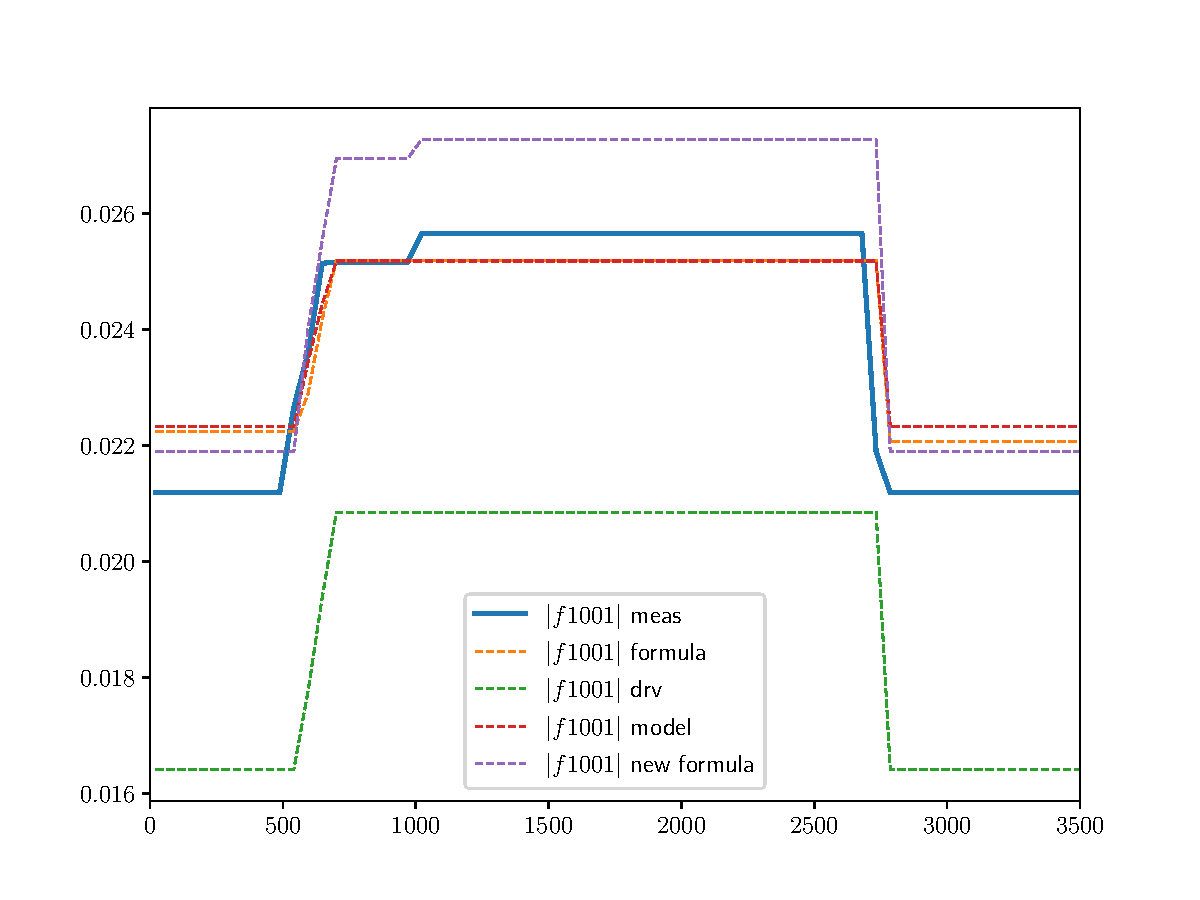
\includegraphics{forced_rdts_abs}
  \caption{Comparison of the three methods with the AC-dipole surrounded by a coupling bump.
    The AC-dipole is creating a jump in the coupling term $f_{1001}$ at its location. Only the new
    formula is able to reproduce this jump.
  }
  \label{fig_comp_felix_ryo}
\end{figure}
%
Figure~\ref{fig_comp_felix_ryo} shows the comparison between the three methods.

